\documentclass[11pt,class=report,crop=false]{standalone}
\usepackage[screen]{../python}
\begin{document}

% Specific command
\newcommand{\badletter}[1]{\underline{\underline{\textcolor{red}{#1}}}}


%====================================================================
\chapitre{Lists I}
%====================================================================

\objectifs{A list is a way to group elements into a single object. After defining a list, you can retrieve each item of the list one by one, but also add new ones\ldots}


%%%%%%%%%%%%%%%%%%%%%%%%%%%%%%%%%%%%%%%%%%%%%%%%%%%%%%%%%%%%%%%%
%%%%%%%%%%%%%%%%%%%%%%%%%%%%%%%%%%%%%%%%%%%%%%%%%%%%%%%%%%%%%%%%

\begin{cours}[List (1)]

A \defi{list}\index{list} is a series of elements. This can be a list of integers, for example \ci{[5,-7,12,99]}, or a list of strings, for example \ci{["March","April","May"]} or objects of different types \ci{[3.14,"pi",10e-3,"x",True]}.

\begin{itemize}
  \item \textbf{Construction of a list.} A list is defined by elements between square brackets:
  \begin{itemize}
    \item \ci{mylist1 = [5,4,3,2,1]} a list of $5$ integers,
    \item \ci{mylist2 = ["Friday","Saturday","Sunday"]} a list of $3$ strings,
    \item \ci{mylist3 = []} the empty list (very useful if you intend to complete the list later).
  \end{itemize}

  \item \textbf{Get an item.} To get an item from the list, simply write \ci{mylist[i]} where $i$ is the rank of the desired item. 
  
  \textbf{Beware!} The trap is that you start counting from the rank $0$. 
  
  For example after the instruction \ci{mylist = ["A","B","C","D","E","F"]} then  
  \begin{itemize}
    \item \ci{mylist[0]} returns \ci{"A"}
    \item \ci{mylist[1]} returns \ci{"B"}
    \item \ci{mylist[2]} returns \ci{"C"}
    \item \ci{mylist[3]} returns \ci{"D"}
    \item \ci{mylist[4]} returns \ci{"E"}
    \item \ci{mylist[5]} returns \ci{"F"}                   
  \end{itemize}  
  
  \medskip
  
 \myfigure{0.4}{
  \tikzinput{fig-lists-1}
}  

  
  \item \textbf{Add an element.} To add an item at the end of a list, just use the command \ci{mylist.append(element)}\index{append@\ci{append}}\index{list!add}. 
  For example if \ci{primes = [2,3,5,7]} then 
  \ci{primes.append(11)} adds $11$ to the list, if you then execute the instruction \ci{primes.append(13)} then the list \ci{primes} becomes  \ci{[2,3,5,7,11,13]}.
  
  \item \textbf{Example of construction.} Here is how to build the list that contains the first ten squares:
   \begin{center}
  \begin{minipage}{0.9\textwidth}
\begin{lstlisting}
list_squares = []            # Start from the empty list
for i in range(10):
    list_squares.append(i**2)   # Add squares one by one
\end{lstlisting}
  \end{minipage}
  \end{center}  
At the end \ci{list_squares} is:
\mycenterline{\ci{[0, 1, 4, 9, 16, 25, 36, 49, 64, 81]}}   
  
         
\end{itemize}
\end{cours}


\begin{cours}[List (2)]
\sauteligne
\begin{itemize}
  \item \textbf{Length of a list.} The length of a list is the number of elements it contains. The command \ci{len(mylist)}\index{len@\ci{len}}\index{list!length} returns the length. The list \ci{[5,4,3,2,1]} is $5$ elements long, the list \ci{["Friday","Saturday","Sunday"]} has length $3$, the empty list \ci{[]} has length $0$.
  
  \item \textbf{Browse a list.} 
	Here is the easiest way to scan a list (and in this case, to display each item):
\begin{lstlisting}
for item in mylist:
    print(item)
\end{lstlisting}

\index{for@\ci{for}}\index{loop!for}

  \item \textbf{Browse a list (again).} 
  Sometimes you need to know the index of the elements. Here is another way to do it (which here displays the index and the element).
\begin{lstlisting}
n = len(mylist)
for i in range(n):
    print(i,mylist[i])
\end{lstlisting}  

\item To get a list from \ci{range()} you have to write:
\mycenterline{\ci{list(range(n))}}

\item It's a bad idea to name your list \og{}\ci{list}\fg{} because this word is already used by \Python{}.
\end{itemize}
\end{cours}



%%%%%%%%%%%%%%%%%%%%%%%%%%%%%%%%%%%%%%%%%%%%%%%%%%%%%%%%%%%%%%%%
% Activity 1
%%%%%%%%%%%%%%%%%%%%%%%%%%%%%%%%%%%%%%%%%%%%%%%%%%%%%%%%%%%%%%%%

\begin{activite}[Simple or compound interests]

\objectifs{Goal: create two lists to compare two types of interests.}
\index{interest}

\begin{enumerate}
  \item \textbf{Simple interest.} We have an amount of $S_0$. Each year this investment earns interest based on the initial amount. 
 
  For example, with an initial amount of $S_0 = 1000$ and simple interest of $p = 10 \%$. The interest is $100$. So after one year, I have a sum of $S_1=1100$, after two years $S_2 = 1200$\ldots
  
  Program a \ci{simple_interest(S0,p,n)} function that returns the list of amounts for the $n$ first years. For example \ci{simple_interest(1000,10,3)} returns 
  \ci{[1000, 1100, 1200, 1300]}.
  
  
  
  \item \textbf{Compound interest.} An amount of $S_0$ brings in compound interest. This time the interest is calculated each year on the basis of the sum of the previous year, i.e. according to the formula: 
  $$I_{n+1} = S_n \times \frac {p}{100}$$
  
    Program a function \ci{compound_interest(S0,p,n)} which returns the list of amounts of the $n$ first years. For example \ci{compound_interest(1000,10,3)} returns 
  \ci{[1000, 1100, 1210, 1331]}.
  
  
  \item I have the choice between a simple interest investment of $10\%$ or a compound interest investment of $7\%$.  What is the most advantageous solution depending on the duration of the placement? 
  
\end{enumerate}

\end{activite}

%%%%%%%%%%%%%%%%%%%%%%%%%%%%%%%%%%%%%%%%%%%%%%%%%%%%%%%%%%%%%%%%
%%%%%%%%%%%%%%%%%%%%%%%%%%%%%%%%%%%%%%%%%%%%%%%%%%%%%%%%%%%%%%%%

\begin{cours}[List (3)]
\sauteligne
\begin{itemize}
  \item \textbf{Concatenate two  lists.}\index{list!merge}\index{concatenation} If you have two lists, you can merge them by the operator \og{}\ci{+}\fg{}. For example with 
  \ci{mylist1 = [4,5,6]} and \ci{mylist2 = [7,8,9]} 
  \mycenterline{\ci{mylist1 + mylist2} \quad is \quad \ci{[4,5,6,7,8,9]}.}
  
    
  \item \textbf{Add an item at the end.}\index{list!add} The operator \og{}\ci{+}\fg{} provides another method to add an item to a list: 
  \mycenterline{\ci{mylist = mylist + [element]}}
  
  For example \ci{[1,2,3,4] + [5]} is \ci{[1,2,3,4,5]}.
  Attention! The element to be added must be surrounded by square brackets.   
  It is an alternative method to \ci{mylist.append(element)}.
  
  \item \textbf{Add an element at the beginning.} With : 
  \mycenterline{\ci{mylist = [element] + mylist}}
  the item is added at the beginning of the list.
  For example \ci{[5] + [1,2,3,4]} is \ci{[5,1,2,3,4]}. 
  
  \item \textbf{Slicing lists.}\index{list!sublist} You can extract a whole part of the list at once: \ci{mylist[a:b]} returns the sublist of items with indices $a$ to $b-1$.
  
  \smallskip
  
 \myfigure{0.4}{
  \tikzinput{fig-lists-3}
}    
  
    For example if \ci{mylist = ["A","B","C","D","E","F","G"]} then  
  \begin{itemize}
    \item \ci{mylist[1:4]} returns \ci{["B","C","D"]}
    \item \ci{mylist[0:2]} returns \ci{["A","B"]}
    \item \ci{mylist[4:7]} returns \ci{["E","F","G"]}
  \end{itemize} 
  Once again, it is important to remember that the index of a list starts at $0$ and that slicing \ci{mylist[a:b]} stops at the rank $b-1$.
   
\end{itemize}
\end{cours}

%%%%%%%%%%%%%%%%%%%%%%%%%%%%%%%%%%%%%%%%%%%%%%%%%%%%%%%%%%%%%%%%
% Activity 2
%%%%%%%%%%%%%%%%%%%%%%%%%%%%%%%%%%%%%%%%%%%%%%%%%%%%%%%%%%%%%%%%

\begin{activite}[Manipulate lists]

\objectifs{Goal: program small routines that manipulate lists.}

\begin{enumerate}
  \item Program a \ci{rotate(mylist)} function that shifts all the elements of a list by one index (the last element becoming the first). The function returns a new list.
  
  For example, \ci{rotate([1,2,3,4])} returns the list \ci{[4,1,2,3]}.
  
  \item Program an \ci{inverse(mylist)} function that inverts the order of the elements in a list. 
  
  For example, \ci{inverse([1,2,3,4])} returns the list \ci{[4,3,2,1]}.
  
  \item Program a \ci{delete_rank(mylist,rank)} function that returns a list of all elements, except the one at the given index. 
  
  For example, \ci{delete_rank([8,7,6,5,4],2)} returns the list \ci{[8,7,5,4]} (item $6$ that was at index $2$ is deleted).
  
    \item Program a \ci{delete_element(mylist,element)} function returning a list that contains all items except those equal to the specified element. 
    
 For example, \ci{delete_element([8,7,4,6,5,4],4)} returns the list \ci{[8,7,6,5]} (all items equal to $4$ have been deleted).
    
\end{enumerate}

\end{activite}



\begin{cours}[Manipulate lists]
  You can now use the \Python{} functions which do some of these operations.
  
\begin{itemize}
  \item \textbf{Invert a list.}\index{list!invert} Here are three methods: \index{reverse@\ci{reverse/reversed}}
\begin{itemize}
  \item \ci{mylist.reverse()} modifies the list in place (i.e. \ci{mylist} is now reversed, the command returns nothing);
  \item \ci{list(reversed(mylist))} returns a new list;
  \item \ci{mylist[::-1]} returns a new list. 
\end{itemize}  

  \item \textbf{Delete an item.}  The command \ci{mylist.remove(element)}\index{list!delete}\index{remove@\ci{remove}} deletes the first occurrence found (the list is modified). For example if \ci{mylist = [2,5,3,8,5]} the call \ci{mylist.remove(5)} modifies the list to become \ci{[2,3,8,5]} (the first $5$ has disappeared).
  
   \item \textbf{Delete an element (again).}  The command \ci{del mylist[i]}\index{del@\ci{del}} deletes the element of rank $i$ (the list is modified).
  
\end{itemize}
\end{cours}



%%%%%%%%%%%%%%%%%%%%%%%%%%%%%%%%%%%%%%%%%%%%%%%%%%%%%%%%%%%%%%%%
% Activity 3
%%%%%%%%%%%%%%%%%%%%%%%%%%%%%%%%%%%%%%%%%%%%%%%%%%%%%%%%%%%%%%%%

\begin{activite}[Bubble sort]

\objectifs{Goal: order a list from the smallest to the largest element.}
%\index{sort}

The bubble sort is a simple way to order a list, here it will be from the smallest to the largest element.
The principle is as follows:
\begin{itemize}
  \item We go through the list from the beginning. As soon as you encounter two consecutive elements in the wrong order, you exchange them. 
  \item At the end of the first pass, the largest element is at the end and it will not move anymore.
  \item We restart from the beginning (until the penultimate element), this time the last two elements are well placed.
  \item We continue this way. There is a total of $n-1$ passages if the list is of length $n$. 
\end{itemize}

 \myfigure{0.7}{
  \tikzinput{fig-lists-2}
} 


\medskip

Here is the bubble sort algorithm:
  \begin{algorithme}
  \sauteligne 
 \begin{itemize}
   \item
   \begin{itemize}
     \item Input: a list $\ell$ of $n$ numbers
     \item Output: the ordered list from the smallest to the largest
   \end{itemize}

   \item For $i$ ranging from $n-1$ to $0$:\\
   \indentation For $j$ ranging from $0$ to $i-1$:\\
   \indentation\indentation If $\ell[j+1] < \ell[j]$ then exchange $\ell[j]$ and $\ell[j+1]$.
   \item Return the list $\ell$.
 \end{itemize}  
 \end{algorithme}
 

Program the bubble sort algorithm into a \ci{bubble_sort(mylist)} function that returns the ordered list of elements. For example \ci{bubble_sort([13,11,7,4,6,8,12,6])} returns the list \ci{[4,6,6,7,8,11,12,13]}.

\medskip

\emph{Hints.}
\begin{itemize}
  \item Begin by defining \ci{new_mylist = list(mylist)} and work only with this new list.
  \item For the index $i$ to run backwards from $n-1$ to $0$, you can use the command: 
\mycenterline{\ci{for i in range(n-1,-1,-1):}}

Indeed \ci{range(a,b,-1)} corresponds to the decreasing list of integers $i$ satisfying $a \ge i > b$ (as usual the right bound is not included).
\end{itemize}

\end{activite}


\begin{cours}[Sorting]

You can now use the \ci{sorted()} function from \Python{} which orders lists.

\index{list!sort}
\index{sorted@\ci{sort/sorted}} 
 
  \begin{fonctionpython}[\ci{python: sorted()}]
    Use: \ci{sorted(mylist)}\\
    Input: a list \\
    Output: the ordered list of elements
  
  \medskip
     
   Example: \ci{sorted([13,11,7,4,6,8,12,6])} returns the list \ci{[4,6,6,7,8,11,12,13]}.

  \end{fonctionpython}  
  
  Attention! There is also a \ci{mylist.sort()} method that works a little differently. This command returns nothing, but on the other hand the list \ci{mylist} is now ordered. We are talking about a modification \emph{in place}.
\end{cours}


%%%%%%%%%%%%%%%%%%%%%%%%%%%%%%%%%%%%%%%%%%%%%%%%%%%%%%%%%%%%%%%%
% Activity 4
%%%%%%%%%%%%%%%%%%%%%%%%%%%%%%%%%%%%%%%%%%%%%%%%%%%%%%%%%%%%%%%%

\begin{activite}[Arithmetic]

\objectifs{Goal: improve some of the \og{}Arithmetic -- While loop -- I\fg{} chapter functions.}

\index{prime number}


\begin{enumerate}
  \item \textbf{Prime factors.}  Program a \ci{prime_factors(n)} function that returns a list of all the prime factors of an integer $n\ge2$. For example, for $n = 12\,936$, its decomposition into prime factors is $n = 2^3 \times 3 \times 7^2 \times 11$, the function returns \ci{[2, 2, 2, 3, 7, 7, 11] }.
  
  \emph{Hints.} Consult the \og{}Arithmetic -- While loop -- I\fg{} chapter. The core of the algorithm is as follows:

\begin{center}
\begin{minipage}{0.7\textwidth}
As long as $d \le n$:\\
\indentation If $d$ is a divisor of $n$, then:\\
\indentation\indentation add $d$ to the list,\\
\indentation\indentation $n$ becomes $n/d$.\\
\indentation Otherwise increment $d$ by $1$.
\end{minipage}
\end{center}

  \item \textbf{List of prime numbers.} Write a \ci{list_primes(n)} function that returns the list of all prime numbers less than $n$. For example \ci{list_primes(100)} returns the list: 
  \mycenterline{\small\ci{[2,3,5,7,11,13,17,19,23,29,31,37,41,43,47,53,59,61,67,71,73,79,83,89,97]}}
  
  To do this, you will program an algorithm that is a simple version of the sieve of Eratosthenes:
  
  \index{sieve of Eratosthenes}
  
  \medskip
  
   \begin{algorithme}
  \sauteligne 
 \begin{itemize}
   \item
   \begin{itemize}
     \item Input: an integer $n \ge 2$.
     \item Ouput: the list of prime numbers $< n$.
   \end{itemize}
   

  
  \item Initialize \ci{mylist} with a list that contains all integers from $2$ to $n-1$. 
   
   \item For $d$ ranging from $2$ to $n-1$:\\
   \indentation For $k$ in \ci{mylist}:\\
   \indentation\indentation If $d$ divides $k$ and $d \neq k$, then
remove the element $k$ from \ci{mylist}.
   \item Return \ci{mylist}.
 \end{itemize}  
 \end{algorithme}
 
 % \medskip

  \emph{Hints.}  
  \begin{itemize}
    \item Start from \ci{mylist = list(range(2,n))}.
    \item Use \ci{mylist.remove(k)}.
   \end{itemize} 
   
   \medskip
   
  \emph{Explanations.}
  Let's see how the algorithm works with $n=30$.
  \begin{itemize}
    \item At the beginning the list is 
    {\small$$ [2,3,4,5,6,7,8,9,10,11,12,13,14,15,16,17,18,19,20,21,22,23,24,25,26,27,28,29]$$
    }
    
    \item We start with $d=2$, we eliminate all the numbers divisible by $2$, unless it is the number $2$: so we eliminate $4$, $6$, $8$,\ldots, the list is now $[2,3,5,7,9,11,13,15,17,19,21,23,25,27,29]$.
    \item We continue with $d=3$, we eliminate multiples of $3$ (except $3$), after these operations the list is: $[2,3,5,7,11,13,17,19,23,25,29]$.
    \item With $d=4$, we eliminate multiples of $4$ (but there are no more).
    \item With $d=5$ we eliminate multiples of $5$ (here we just eliminate $25$), the list becomes $[2,3,5,7,11,13,17,19,23,29]$.
    \item We continue (here nothing happens anymore).
    
    \item At the end, the list is $[2,3,5,7,11,13,17,19,23,29]$.
  \end{itemize}
     
\end{enumerate}

\end{activite}



%%%%%%%%%%%%%%%%%%%%%%%%%%%%%%%%%%%%%%%%%%%%%%%%%%%%%%%%%%%%%%%%
%%%%%%%%%%%%%%%%%%%%%%%%%%%%%%%%%%%%%%%%%%%%%%%%%%%%%%%%%%%%%%%%

\begin{cours}[Plot a list]

With the \ci{matplotlib} module it is very easy to visualize the elements of a list of numbers.

\index{matplolib@\ci{matplotlib}}
\index{module!matplolib@\ci{matplotlib}}
%\index{plot}

\begin{center}
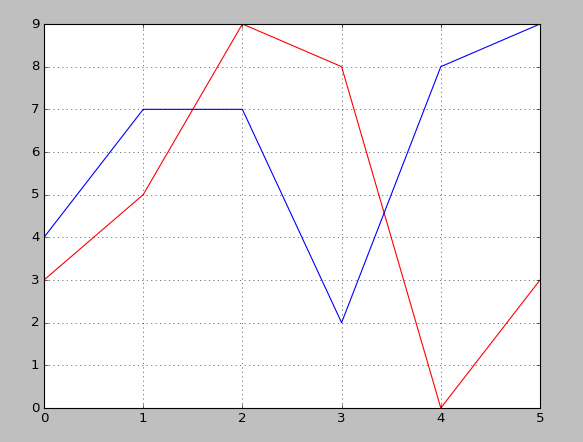
\includegraphics[scale=\myscale,scale=0.45]{screen-lists-lesson-visualization}
\end{center}

\begin{lstlisting}
import matplotlib.pyplot as plt

mylist1 = [3,5,9,8,0,3]
mylist2 = [4,7,7,2,8,9]

plt.plot(mylist1,color="red")
plt.plot(mylist2,color="blue")
plt.grid()
plt.show()
\end{lstlisting}


\emph{Explanations.}
\begin{itemize}
  \item The module is named \ci{matplotlib.pyplot} and is given the new simpler name of \ci{plt}.
  
  \item Attention! The \ci{matplotlib} module is not always installed by default with \Python.
  
  \item \ci{plt.plot(mylist)}\index{plot@\ci{plot}} traces the points of a list (in the form of $(i,\ell_i)$) that are linked by segments.
  
  \item \ci{plt.grid()} draws a grid.
  
  \item \ci{plt.show()} displays everything.  
  
\end{itemize}

\bigskip

To display points $(x_i,y_i)$ you must provide the list of $x$-values then the list of $y$-values:
\mycenterline{\ci{plt.plot(mylist_x,mylist_y,color="red")}}
Here is an example of a graph obtained by displaying coordinate points of the type $(x,y)$ with $y = x^2$.

\begin{center}
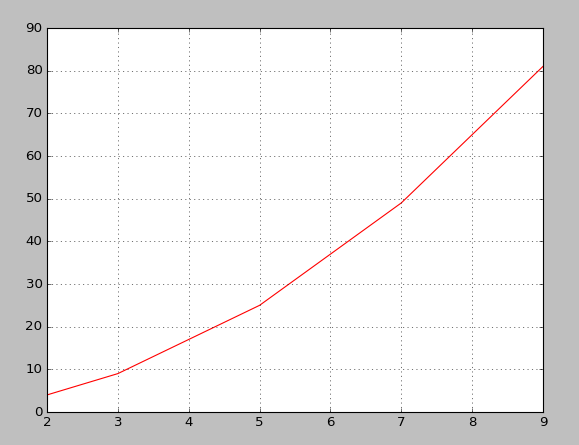
\includegraphics[scale=\myscale,scale=0.45]{screen-lists-lesson-visualization-bis}
\end{center}


\begin{lstlisting}
import matplotlib.pyplot as plt

mylist_x = [2, 3, 5, 7, 9]
mylist_y = [4, 9, 25, 49, 81]
plt.plot(mylist_x,mylist_y,color="red")
plt.grid()
plt.show()
\end{lstlisting}

\end{cours}


%%%%%%%%%%%%%%%%%%%%%%%%%%%%%%%%%%%%%%%%%%%%%%%%%%%%%%%%%%%%%%%%
% Activity 5
%%%%%%%%%%%%%%%%%%%%%%%%%%%%%%%%%%%%%%%%%%%%%%%%%%%%%%%%%%%%%%%%

\begin{activite}[Ballistics]

\objectifs{Goal: visualize the firing of a cannonball.}

\index{ballistics}

\begin{center}
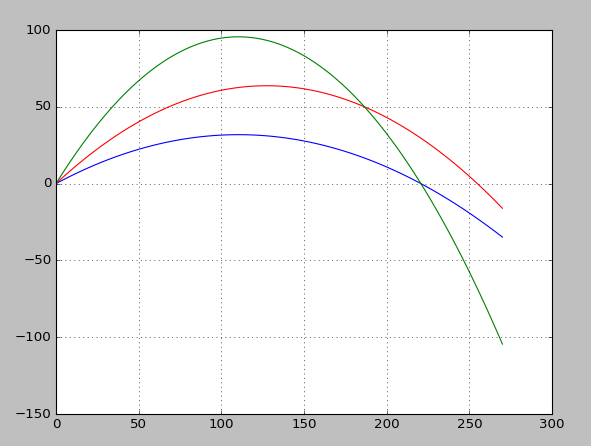
\includegraphics[scale=\myscale,scale=0.45]{screen-lists-I-tir-bis}
\end{center}

A cannonball has been fired from the point $(0,0)$. The trajectory equation is given by the formula:
$$y(x) = -\frac12  g \frac{1}{v^2 \cos^2(\alpha)} x^2 \  + \   \tan (\alpha)  x$$
where
\begin{itemize}
  \item $\alpha$ is the angle of the shot,
  \item $v$ is the initial speed,
  \item $g$ is the gravitational constant: we will take $g = 9.81$.
\end{itemize}

\myfigure{0.7}{
  \tikzinput{fig-lists-I-tir}
} 

\begin{enumerate}
  \item Program a \ci{parabolic_shot(x,v,alpha)} function
  which returns the value $y(x)$ given by the formula.
  
  \emph{Hint.} Be careful with the units for the angle $\alpha$. If for example you choose that the unit for the angle is degrees, then to apply the formula with \Python{} you must first convert the angles to radians :
  $$\alpha_{\text{radian}} = \frac{2\pi}{360} \alpha_{\text{degree}}$$
  
  \item Program a \ci{list_trajectory(xmax,n,v,alpha)} function that calculates the list of $y$-values of the $n+1$ points of the trajectory whose $x$-values are regularly spaced between $0$ and $x_{\max}$. 
  
  \emph{Method.} For $i$ ranging from $0$ to $n$:
  \begin{itemize}
    \item calculate $x_i = i \cdot \frac{x_{\max}}{n}$,    
    \item calculate $y_i = y(x_i)$ using the trajectory formula,
    \item add $y_i$ to the list.
  \end{itemize}  
  
  
  \item For $v=50$, $x_{\max} = 270$ and $n=100$, display different trajectories according to the values of $\alpha$. What angle $\alpha$ allows to reach the point $(x,0)$ at ground level as far away from the shooting point as possible?
  
% \emph{Caution !} On the figure displayed by \Python, the data entered in abscissa corresponds to the rank $i$ of the suite and not to the value $x$.
  
\end{enumerate}

\end{activite}


\end{document}
